\tikzstyle{rblock} = [rectangle, draw, text width=15em, text centered, inner sep=0pt, minimum height=2em, rounded corners]
\tikzstyle{line} = [draw, -latex']
\tikzstyle{arrow} = [thick,->,>=stealth]

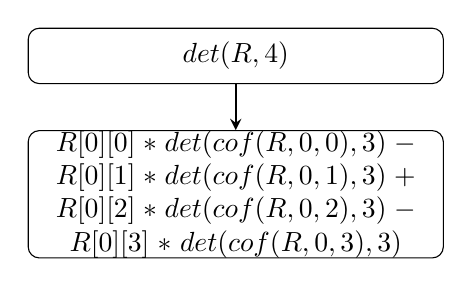
\begin{tikzpicture}[node distance = 5em, auto]
    \node (node1) [rblock] {$det(R, 4)$};
    \node (node2) [rblock, below of = node1] {$R[0][0] * det(cof(R, 0, 0), 3) - R[0][1] * det(cof(R, 0, 1), 3) + R[0][2] * det(cof(R, 0, 2), 3) - R[0][3] * det(cof(R, 0, 3), 3)$};
    \draw [arrow] (node1) -- (node2);
\end{tikzpicture}